\chapter{Related Work}
\label{chapter_2} In this chapter we present an overview of the
previous related works. We start by reviewing the literature for
facial features extraction from frontal 2-D images and 3-D range
images. Afterwards, we review the literature for 2-D and 3-D face
recognition. Finally we review the algorithms for multi-modal (2-D +
3-D) face recognition.

\section{Facial Features Extraction}
In both 2-D and 3-D face recognition systems, alignment
(registration) between the query and the template images or models
is necessary \cite{shan04}. This is the main step before recognition
in a typical face recognition system. This step is usually based on
extracted facial features (i.e., fiducial points). Figure
\ref{fig:facial_features_sample} shows a sample of labeled facial
features on both frontal and profile face images. Beside the
applications of facial features extraction for face recognition,
other applications such as tracking, expression analysis, and
animation rely on facial features extraction. Automatic extraction
of facial features has been one of the important and challenging
tasks and many approaches and algorithms have been developed and
presented for facial features extraction. Many of these methods are
cited and reviewed in face detection and face recognition surveys
\cite{FaceRecoSurvey2003, chellappa95, yang02}.

\bfig \epsfig{figure = ./chapters/figures/facial_features.eps, scale
= 0.7} \caption{Labeled facial features in frontal and profile
images.} \label{fig:facial_features_sample}\efig

In this Section, we review the most important algorithms and methods
for 2-D and 3-D facial features extraction.
\subsection{2-D Facial Features Extraction From Frontal Images}
Facial features extraction is defined as the process of locating
specific region, points, landmarks, or curves/contours in a given
2-D image or a 3-D range image
\cite{ffe1,ffe2,ffe3,ffe4,ffe5,ffe6,ffe7,ffe8}. Although many facial
feature extraction algorithms have been proposed so far, facial
feature extraction is difficult to the applications due to its high
complexity. The computational cost of facial features extraction is
dominated by the localization of the face region and the searching
for the feature points. Generic methods extract features from images
without relying on extensive knowledge about the object of interest.
They have the advantage of being typically fast and simple. However,
these approaches can become unreliable when the quality of the image
is poor or the face in the image has a cluttered background. The
algorithms for facial feature extraction can be divided into four
types:
%%%
\bn

\item Generic methods based on edges, lines, and curves.

\item Template-based methods that are used to detect
facial features such as the eyes.

\item Structural matching methods that take into consideration
the geometrical constraints on the features (i.e. everyone has two
eyes above the mouth).

\item Hybrid methods which combine some of the above previous
methods. \en

Table \ref{tab:facial_features_survey} reviews some of the important
published methods for 2-D facial features extraction from frontal
images.

\btable{\scriptsize
\setstretch{1}\bt{|p{1in}|p{0.75in}|p{1.2in}|p{1.2in}|p{0.75in}|}
\hline
\textbf{Author} & \textbf{Face detection} & \textbf{Approach} & \textbf{Number of feature points} & \textbf{Video/Still}\\
\hline

S. Kobayashi \etal 1995 \cite{ffe1} & Included  &  Using
spatiotemporal difference image to extract the feature points &
Representing eyes, eyebrows, boundary, mouth and face boundary by
contours  & Video - Frontal
\\ \hline
T.F. Cootes \etal 1996 \cite{Cootes_1, Cootes_2}& - &  Using active
shape models& Flexible in term of number of features & Still -
Frontal
\\ \hline

F.G.B. De Natalie 1997 \cite{ffe2} & Included & Identification of
the face symmetry axis and then feature points using correlation &
Location of eyes, and mouth & Still - Frontal

\\ \hline
A. Nikoladis 1997 \cite{ffe3} &  Included & Using adaptive Hough
transform, template matching and active contour models & Eyes,
eyebrows, mouth, nostrils, cheeks and chin  &  Still - Frontal
\\ \hline
K. Lam and Y. Li \etal 1998 \cite{ffe9} & - & Eye corner detection
and template matching  & Eyes &   Still - frontal
\\ \hline
Y. Yagi 2000 \cite{ffe10} & Included & - & Pupil, and contours &
Still - Frontal
\\ \hline
C.M. Lau \etal 2001 \cite{ffe4} & Included &  Using energy function
to extract facial features &   Face region, iris,  eyebrows, nose,
mouth, eye corners, face-hair  & Still - Frontal
\\ \hline

G. Yen and N. Nithianandan 2002  \cite{ffe5} &  Included  &  Using
the edge density distribution of the image and genetic algorithm  &
Face region, eyes, nose, mouth & Still - Frontal
\\ \hline

K. Seo \etal 2002 \cite{ffe6} & Included & Using active contour
model and color information  &  Face region, eyes, nose, mouth &
Still - Frontal
\\ \hline

D. Xi and S.W. Lee \etal 2003 \cite{ffe7} & Included & Using Support
Vector Machines and Multi wavelet decomposition   & Face region,
eyes, nose, mouth & Still - Frontal
\\ \hline
Z. Xue \etal 2002 \cite{ffe11} &  -  & Using Bayesian shape model &
A mesh model of facial features & Still - Frontal
\\ \hline

R. Hsu \etal 2002 \cite{Mottaleb02}  & Included  &  Using color
information for face detection & Face boundary, eyes, mouth&  Still
- Frontal with pose
\\ \hline

Y. Hu \etal 2003 \cite{ffe12} &  -  & Using linear combination model
& Eyes, eyebrows, nose, mouth & Still - Frontal

\\ \hline
A. Gundaz and H. Krim 2003 \cite{ffe13} &  -  & Using topological
operators & Eye corners and mouth center &  Still - Frontal
\\ \hline
K. Kim \etal 2004 \cite{ffe8} & -  & Using PCA and Wavelet multi
resolution images  & Eyes, eyebrows, nose, mouth & Still - Frontal
\\ \hline
K. Nagao 2004 \cite{ffe14} &  -  & Using Bayesian approach with
nonlinear kernels  & Eye centers & Still - Frontal with pose

\\ \hline

\et} \caption{Facial features extraction techniques.}
\label{tab:facial_features_survey} \etable

%%%%%%%%%%%%%
Kobayashi \etal \cite{ffe1} described an automated algorithm for
face detection and facial features extraction from video images. The
extracted features are points around the eyes, mouth, nose and
facial contours. The authors used spatiotemporal difference images
to extract these feature points. For example blinking is used for
detecting the eyes. The method proposed by De Natalie \etal
\cite{ffe2} aimed at identifying the position of characteristic
facial elements (eyes, nose and mouth). The proposed detection
strategy is based on the identification of the face symmetry axis,
and the successive detection of eyes, mouth and other relevant
facial features using correlation.

Nikolaidis \etal \cite{ffe3} described a method for extracting
facial features with the goal of using them in defining a sufficient
set of distances between them so that a unique description of the
structure of a face is obtained. Eyebrows, eyes, nostrils, mouth,
cheeks and chin are considered as interesting features. Candidates
for eyes, nostrils and mouth are determined by searching for minima
and maxima in the $x$ and $y$ projections of the gray level pixels
in the image. Candidates for cheeks and chin are determined by
performing adaptive hough transform on a sub-image defined according
to the position of the eyes, mouth, and the ellipse containing the
main connected component of the image. In order to acquire a more
accurate model of the face, a deforming technique is also applied to
the ellipse representing the main face region. Candidates for
eyebrows are determined by adapting a proper gray level template to
an area restricted by the position of the eyes.

Lam \etal \cite{ffe9} devised an efficient approach for detecting
and locating the eyes in frontal images. Possible eye candidates in
an image are identified by means of the valley features and corners
of the eyes. Two possible eye candidates are considered to belong to
the eyes of a human face if their respective local properties are
similar; an eye window is then formed. Each eye region candidate is
then further verified by comparison with a standard eye template,
and by measuring its symmetry. Yagi \cite{ffe10} presented a system
that integrates a library of 32 functions for automatic facial
contour extraction. The 32 functions can be classified into five
groups such as face detection, pupil detection, facial parts
detection, facial parts contour extraction, and face contour
extraction. The system is not only useful for automatic 3-D facial
model fitting, but also for range facial image processing
applications such as personal authentication and facial expression
analysis. Lau \etal \cite{ffe4} proposed an energy function which is
the sum of seven weighted terms for facial features extraction. By
allocating different values for the weighting factors, the function
can extract different fiducial points.

Yen \etal \cite{ffe5} presented a method for facial features
extraction that uses the edge density distribution of the image. In
the preprocessing stage, a face is approximated by an ellipse, and a
genetic algorithm is applied to search for the best matching region.
In the feature extraction stage, a genetic algorithm is applied to
extract the facial features, such as the eyes, nose and mouth, in
the predefined sub regions. The authors validated their method by
experimenting on various video images under natural lighting
environments and in the presence of noise and different face
orientations.

Seo \etal \cite{ffe6} presented an active contour model based upon
color information for extracting facial features. Their algorithm is
composed of three main parts: the face region estimation part, the
detection part and the facial features extraction part. In the face
region estimation part, images are segmented based on human skin
color. In the face detection part, a template matching method is
used, and in the facial features extraction part, an algorithm
called ``color snake'' is applied to extract facial feature points
within the estimated face region.

Xi \etal \cite{ffe7} developed an algorithm for detecting human face
and extracting facial features based on several support vector
machines. A face model for both detection and extraction was
designed based on multi-resolution wavelet decomposition (MWD). The
MWD and a small number of feature points were applied to roughly
detect the face. More accurate results were achieved by a series of
support vector machines. Xue \etal \cite{ffe11} presented a novel
application of the Bayesian Shape Model (BSM) for facial features
extraction. First, a full-face model is designed to describe the
shape of a face, and the PCA is used to estimate the shape variance
of the face model. Then, the BSM is applied to match and extract the
face patch from input face images. Finally, using the face model,
the extracted face patches are easily warped or normalized to a
standard view.

Hsu \etal \cite{Mottaleb02} proposed a face detection algorithm from
color images in the presence of varying lighting conditions as well
as complex backgrounds. Based on a novel lighting compensation
technique and a nonlinear color transformation, this method detects
skin regions over the entire image and then generates face
candidates based on the spatial arrangement of these skin patches.
The algorithm constructs eye, mouth, and boundary maps for verifying
each face candidate. Hu \etal \cite{ffe12} proposed a facial feature
extraction method based on a linear combination model. The model
uses the knowledge of prototype faces, which are manually labeled,
to interpret novel faces. Generally, the construction of the linear
combination model depends on pixel-wise alignments of prototypes,
and the alignments are computed by an optical flow algorithm or
bootstrapping algorithm which is a full-scale optimization and
without including local information such as facial feature points.
To combine local facial features with the linear combination model,
an optical flow algorithm is proposed to compute the pixel-wise
alignments.

Gundaz \etal \cite{ffe13} presented a method for facial features
extraction by considering the face image as a surface. Topological
properties of the facial surface, such as principal curvatures are
used to extract the eyes and mouth, which form deep valleys on the
surface. The basic idea of the proposed method is to model the
facial features as ravines on the facial surface. Ravines are points
on the surface where the maximum curvature is a local maximum in the
corresponding principal direction. Kim \etal \cite{ffe8} proposed an
algorithm for extracting facial feature fields (eyebrow, eye, nose,
and mouth) from gray scale face images. The foundation of this
method is that eigenfeatures, derived from the eigenvalues and
eigenvectors of the gray scale data set constructed from the feature
fields, are very useful to locate these fields efficiently. In
addition, multi-resolution images, derived from a 2-D DWT (Discrete
Wavelet Transform), are used to reduce the search time for the
facial features. Nagao \cite{ffe14} described a method for finding
the positions of features in facial images. A large class of image
variations, including those resulting from object rotation in 3-D
space and scaling (i.e., translation in depth), are handled. A MAP
(Maximum a Posteriori) estimation technique using Gaussian
distribution is exploited to model the relationship between images
and feature positions.

Deformable models used for non-rigid object segmentation, received
attention in recent years. These models have proven to be efficient
in many applications such as object segmentation, appearance
interpretation, motion tracking etc. A deformable model can be
characterized as a model, which under an implicit or explicit
optimization criterion deforms to match the shape of a known object
in a given image. For a general review of the most commonly used
models, we refer the readers to \cite{McInerney96, Jain98}.

In this dissertation, we improve the Active Shape Model (ASM) for
facial features extraction. The original ASM developed by Cootes
\etal \cite{Cootes_1} suffers from factors such as, poor model
initialization, intensity modeling of the local structure of the
facial features, and alignment of the shape model to a new instant
of the object in a given image using simple similarity
transformation. The core of our enhancement relies on three
improvements (a) initializing the ASM model using a given set of
points (e.g., the centers of the mouth and eyes, which are located
using color information), (b) incorporating color information to
represent the local structure of the feature points, and (c)
applying 2-D affine transformation in aligning the facial features
that are perturbed by head pose variations, which effectively aligns
the matched facial features to the shape model and compensates for
the effect of the head pose variations. The details of our improved
Active Shape Model (ASM) for facial features extraction are
presented in Chapter 3.

\subsection{3-D Facial Features Extraction}
The previous works that utilized 3-D features for face recognition
can be categorized into four groups:

\begin{enumerate}

\item Curvature-based methods.

\item Direct spatial surface matching.

\item Shape representation-based methods.

\item Multi-modal based methods that combines information from 2-D intensity images with 3-D range images.

\end{enumerate}
Most of the early studies concentrate on curvature analysis. In
\cite{gordon91}, the surface regions from range images are
classified as convex, concave, and saddle by calculating the minimum
and maximum principal curvature. Then locations of facial features
are determined, which are used for template comparison. Lee \etal
\cite{lee90} detects corresponding regions in two range images by
graph matching based on Extended Gaussian Image (EGI). Tanaka \etal
\cite{tanaka98} also use EGI. For each face, two EGIs are
constructed from maximum principal direction and minimum principal
direction. The EGI similarity is measured by Fisher's spherical
correlation. In spatial matching approaches, recognition is achieved
via matching facial surfaces directly in 3-D Euclidean space
\cite{Beumier00,pan03}. In shape representation methods, the 3-D
facial shape or surface is converted to another shape representation
such as point signature (PS) \cite{chua00}, spin image (SP)
\cite{Johnson99}, shape distribution \cite{Osada02}, or Local Shape
Map (LSM) \cite{wu04}. LSM is based on point signature approach and
spin images. Thus the recognition task can be achieved in the
representation domain.

Johnson \etal \cite{Johnson99} compute a spin image which describes
the shape of the surface. It is created by projecting a surface 3-D
point $P$ onto 2-D coordinates via a spin map function S using
oriented point on the surface. The oriented point is the coordinate
location on the surface with the normal, i.e., $(x,y,n)$. An image
is created by applying $S$ to all points on the surface. This image
can be used in object recognition or 3-D surface registration. Point
signature encodes a surface point $p$ in a predefined periphery to a
tangential plane, $P$ passing through $p$  \cite{chua00}. Neighbors
of point $p$ are found by intersecting the original surface with a
sphere. $P$ is formed by fitting a plane to the neighboring points,
and by translating it to the original point $p$. Signed distances
are sampled by $\Delta\theta$ degree intervals, thus forming a 1D
parametric curve, $d(\theta)$. In the recognition phase, each point
signature extracted from the test image is compared with each
image's point signatures, for the database images and a total
similarity between the database and the probe image is computed
according to the sum of individual point signature distances.

The facial structure can also be described with the aid of 2-D or
3-D data sources. Assisted by a statistical feature location model,
Lu \etal \cite{lu05_techrep} automatically combine 3-D features
shape index response, derived from the range map, with 2-D intensity
corner-ness response to determine the correct positions of the
corners of the eyes and the mouth. A feature extractor based on the
directional maximum is presented to estimate the tip of the nose and
the pose angle simultaneously. In other words, the nose tip has the
largest depth value if projected onto the corrected pose direction.
The limitation of the nose extraction approach is due to not making
full use of the entire 3-D directional rotations (rotation about the
$z$ and $x$) and only yaw pose variation (rotation about the
$y$-axis) is assumed. Similarly, Wang \etal \cite{wang02} showed
that by combining 2-D Gabor wavelet-based image intensity features
with point signature-based 3-D shape features they obtained a
superior performance than using each modality alone.

In Chapter 3, we present an algorithm based on Gaussian curvature to
extract three feature points which are utilized in face alignment
during the recognition process. The extracted feature points are the
two inner corners of the eyes and the tip of the nose. Before
extracting the facial features from 3-D range data, we locate the
face in the range image and only keep the face areas and exclude the
background, hair, and neck in the image. Therefore, we developed a
method for localizing faces in range data using template matching.

\section{Face Recognition}
A man-machine facial recognition system dates way back to 1965
\cite{chan65}. The authors showed that a computer program provided
with facial features extracted manually could perform recognition
with satisfactory performance. In the past few years, face
recognition has received great attention. A recent literature survey
of face recognition is given in \cite{FaceRecoSurvey2003}, where
most of the paper surveys 2-D algorithms. In addition, the work and
survey by Bowyer \etal \cite{bowyer04} in 2004 gives a comparison
among face recognition techniques based on 2-D data, 3-D data, and
2-D + 3-D data fusion. They reported that 3-D face recognition
approaches outperform 2-D approaches and the fusion of 2-D + 3-D
data produces slightly better results than 3-D alone. A very recent
survey by Bowyer \etal \cite{3DFaceSurvey2006} in 2006 cited some
approaches that some 2-D recognition approaches outperform 3-D
approaches. There is a belief that it is still premature to make
this judgment at this time because current approaches did not yet
make full use of 3-D data either in the recognition algorithms or
the rigorous experimental methodology.

\subsection{2-D face Recognition}
Many algorithms for face recognition have been proposed during the
past three decades. The literature on face recognition is vast and
diverse. Zhao \etal  \cite{FaceRecoSurvey2003} presented a
literature survey of 2-D face recognition. We refer the readers to
this paper for a complete survey of the state of the art in the area
of 2-D face recognition. In this Section, we review the important
approaches for 2-D face recognition.

The algorithms for 2-D face recognition are divided into three
categories in \cite{FaceRecoSurvey2003}. This is a clear and
high-level categorization based on a guideline suggested by the
psychological study of how humans use holistic and local features
\cite{FaceRecoSurvey2003}.

\begin{enumerate}

\item \textit{Holistic matching methods}: These methods use the whole face region
as the raw input to a recognition system. One of the most widely
used representations of the face region is eigenfaces
\cite{Eigenface1991}, which are based on principal component
analysis.

\item

\textit{Feature-based (structural) matching methods}: Typically, in
these methods, local features such as the eyes, nose, and mouth are
first extracted and their locations and local statistics (geometric
and/or appearance) are fed into a structural classifier.

\item
\textit{Hybrid methods}: Just as the human perception system uses
both local features and the whole face region to recognize a face, a
machine recognition system should use both. One can argue that these
methods could potentially offer the best of the two types of
methods.

\end{enumerate}

Table \ref{tab:2-D face_recognition} classifies each category into
sub-classes. In the following subsections, we review in details the
most important methods in each class.

\btable{\scriptsize \setstretch{1.5}\bt{|p{2in} p{3.5in}|} \hline
\textbf{Approach} &
\textbf{Works}\\
\hline \textbf{Holistic methods} & \\
~~~\textit{Principal component analysis (PCA)} &\\
~~~~~Eigenfaces & Direct application of PCA \cite{kirby90, Eigenface1991}\\
~~~~~Bayesian & Two-class problem with probability measure \cite{moghaddam97}\\
~~~~~Fisherfaces/LDA & FLD on eigenspcace \cite{Belhumeur97, zhao98, Swets96_b}\\
~~~~~ICA & ICA-based feature analysis \cite{Bartlett98}\\
~~~\textit{Other representations} & Neural Network based method
\cite{Lin97}
\\ \hline
\textbf{Feature-based methods} & \\
~~~Pure geometry methods & Earlier works \cite{kanade77, kelly70}\\
~~~Dynamic link architecture & Elastic Graph Matching \cite{Okada98, Wiskott97, bolme_03}\\
~~~Hidden Markov model & HMM methods\cite{Samaria94_a, Samaria94_b}
\\ \hline

\textbf{Hybrid methods} & \\
~~~Modular eigenfaces & Eigenfaces and egienmodules \cite{pentland94}\\
~~~Hybrid LFA & Local feature method \cite{penev96}\\
~~~Shape Normalized & Flexible appearance models \cite{lanitis95}\\

\hline \et} \caption{Classification of 2-D face recognition
techniques \cite{FaceRecoSurvey2003}.} \label{tab:2-D
face_recognition} \etable

\subsection{Holistic-based Approaches}
\subsubsection{Principal Component Analysis}
Successful low-dimensional representation of faces using
Kullback-Leibler (KL) or Principal Component Analysis (PCA)
projections starts from the works by Kirby and Sirovich in 1987
\cite{sirovich87} and 1990 \cite{kirby90}. Eigenpictures have been
one of the major driving forces behind face representation,
detection, and recognition. It is well known that there exist
significant statistical redundancies in natural images
\cite{ruderman94}. For a limited class of objects such as face
images that are normalized with respect to scale, translation, and
rotation, the redundancy is even greater \cite{penev96,
zhao99_thesis}. One of the best global compact representations is
KL/PCA, which decorrelates the outputs. More specifically, sample
vectors $x$ can be expressed as linear combinations of the
orthogonal basis $\Phi_i$:

\beq x = \sum_{i=1}^{n}a_i\Phi_i \approx \sum_{i=1}^{m}a_i\Phi_i
\eeq where typically $m \ll n$. The basis $\Phi_i$ are calculated by
solving the eigenproblem:

\beq
 C\Phi = \Phi \Lambda
\eeq where $C$ is the covariance matrix for input $x$.

Such representation is less sensitive to noise that may be due to
small occlusions, as long as the topological structure does not
change.

Turk and Pentland \cite{Eigenface1991} made a very successful
demonstration of machine recognition on faces using eigenpictures
(known as eigenfaces) for face detection and identification. Figure
\ref{fig:EigenFace} shows an example of eigenfaces. Given the
eigenfaces, every face in the database can be represented as a
vector of weights; the weights are obtained by projecting the image
into eigenface components by a simple inner product operation. When
a new test image whose identification is required is given, the new
image is also represented by its vector of weights. The
identification of a face image is done by locating the image in the
database whose weights are the closest to the weights of the test
image.

\bfig \epsfig{figure = ./chapters/figures/eigenface.eps, scale =
0.5} \caption{Example of eigenfaces.} \label{fig:EigenFace}\efig

Moghaddam and Pentland \cite{moghaddam97} extended the standard
eigenface approach to a Bayesian approach. They used a probabilistic
measure of similarity, instead of the simple Euclidean distance used
with eigenfaces in \cite{Eigenface1991}. The major drawback of a
Bayesian method is the need to estimate probability distributions in
a high-dimensional space from a very limited number of training
samples per class. To avoid this problem, a much simpler two-class
problem was created from the multi-class problem. Two mutually
exclusive classes were defined: $\Omega_I$, representing
intra-personal variations between multiple images of the same
individual, and $\Omega_E$, representing extra-personal variations
due to differences in identity. Assuming that both classes are
Gaussian-distributed, likelihood functions $P(\Delta|\Omega_I)$ and
$P(\Delta|\Omega_E)$ were estimated for a given intensity difference
$\Delta = I_1 - I_2$. Given these likelihood functions and using the
MAP rule, two face images are determined to belong to the same
individual if $P(\Delta|I) > P(\Delta|E)$. A large performance
improvement of this probabilistic matching technique over standard
nearest-neighbor eigenspace matching was reported using large face
data sets including the FERET database \cite{FERET2000}.

Successful face recognition systems using Linear Discriminant
Analysis/Fisher Linear Discriminant (LDA/FLD) were reported by
\cite{Belhumeur97, Etemad97, Swets96_b, zhao98, zhao99}. LDA
training is carried out via scatter matrix analysis
\cite{fukunaga89}. For an $M-$class problem, the within- and
between-class scatter matrices $S_w$, $S_b$ are computed as follows:

\beq
 S_w = \sum_{i=1}^M Pr(\omega_i)C_i ,\\
 S_b = \sum_{i=1}^M Pr(\omega_i)(m_i - m_0)(m_i - m_0)^t,
\eeq where $Pr(\omega_i)$ is the prior class probability, and is
usually replaced by $1/M$ in practice with the assumption of equal
priors. Here $S_w$ is the within-class scatter matrix, showing the
average scatter $C_i$ of the sample vectors $x$ of different classes
$\omega_i$ around their respective means $m_i$:

\beq C_i = E[(x(\omega)- m_i)(x(\omega) - m_i)^t|\omega = \omega_i].
\eeq

Similarly, $S_b$ is the Between-class Scatter Matrix, representing
the scatter of the conditional mean vectors $m_i$ around the overall
mean vector $m_0$. A commonly used measure for quantifying
discriminatory power is the ratio of the determinant of the
between-class scatter matrix of the projected samples to the
determinant of the within-class scatter matrix:

\beq \mathcal{J}(T) = |T^t S_bT|/|T^tS_wT|. \eeq

The optimal projection matrix W which maximizes $\mathcal{J}(T)$ can
be obtained by solving a generalized eigenvalue problem:

\beq S_bW = S_wW \Lambda_W. \eeq

It is helpful to make comparisons among the so-called (linear)
projection algorithms. Here we illustrate the comparison between
eigenfaces and Fisherfaces. Similar comparisons can be made for
other methods, for example, ICA projection methods. In all these
projection algorithms, classification is performed by (1) projecting
the input $x$ into a subspace via a projection/basis matrix
$P_{roj}$:

\beq z = P_{roj}x \eeq (2) comparing the projection coefficient
vector $z$ of the input to all the pre-stored projection vectors of
labeled classes to determine the input class label. The vector
comparison varies in different implementations and can influence the
system's performance dramatically \cite{Moon01}. For example, PCA
algorithms can use either the angle or the Euclidean distance
(weighted or unweighted) between two projection vectors. For LDA
algorithms, the distance can be unweighted or weighted.

A comparative performance analysis was carried out by Belhumeur
\etal \cite{Belhumeur97}. They compared four methods: (1) a
correlation-based method, (2) a variant of the linear subspace
method suggested in \cite{Shashua94}, (3) an eigenface method by
Turk and Pentland \cite{Eigenface1991}, and (4) a Fisherface method
which uses subspace projection prior to LDA projection to avoid the
possible singularity in $S_w$ as in \cite{Swets96_b}. Experiments
were performed on a database of 500 images created by
\cite{Hallianan94} and a database of 176 images created at Yale
\cite{yale_faceDatabase}. The results of the experiments showed that
the Fisherface method performed significantly better than the other
three methods. However, no claim was made about the relative
performance of these algorithms on larger databases.

Bartlett \etal \cite{Bartlett98} presented an argument that for
tasks such as face recognition, much of the important information is
contained in high-order statistics. So, they proposed to use
independent component analysis (ICA) to extract features for face
recognition. ICA is a generalization of principal component
analysis, which decorrelates the high-order moments of the input in
addition to the second-order moments.

\subsubsection{Neural Network-based Approaches}
A fully automatic face detection/recognition system based on a
neural network is reported in \cite{Lin97}. The proposed system is
based on a probabilistic decision-based neural network (PDBNN, an
extended (DBNN) \cite{Kung95}) which consists of three modules: a
face detector, an eye localizer, and a face recognizer. Unlike most
methods, the facial regions contain the eyebrows, eyes, and nose,
but not the mouth. The rationale of using only the upper face is to
build a robust system that excludes the influence of facial
variations due to expressions that cause motion around the mouth. To
improve robustness, the segmented facial region images are first
processed to produce two features at a reduced resolution of
$14�10$: normalized intensity features and edge features, both in
the range $(0, 1)$. These features are fed into two PDBNNs and the
final recognition result is the fusion of the outputs of these two
PDBNNs.

Compared to most multi-class recognition systems that use a
discrimination function between any two classes, PDBNN has a lower
false acceptance/rejection rate because it uses the full density
description for each class. In addition, this architecture is
suitable for hardware implementation such as distributed computing.
However, it is not clear how to accurately estimate the full density
functions for the classes when there are only limited numbers of
samples. Further, the system could have problems when the number of
classes grows exponentially.

\subsection{Geometric-based Approaches}
Many methods in the geometric matching category have been proposed,
including early methods based on geometry of local features
\cite{kanade77,kelly70} as well as 1D \cite{Samaria94_a} and
pseudo-2-D \cite{Samaria94_b} HMM methods. One of the most
successful of these systems is the Elastic Bunch Graph Matching
(EBGM) system \cite{Okada98, Wiskott97}, which is based on Dynamic
Link Architecture (DLA) \cite{Buhmann90, Lades93}. Gabor wavelets
play a building block role for facial representation in these graph
matching methods. A typical local feature representation consists of
wavelet coefficients for different scales and rotations based on
fixed wavelet bases (called jets in \cite{Okada98}). These locally
estimated wavelet coefficients are robust to illumination change,
translation, distortion, rotation, and scaling. The basic 2-D Gabor
function and its Fourier transform are

\beq g(x, y : u_0, v_0) = exp(-[x^2/2\sigma_x^2 + y^2/2\sigma_y^2]+ 2\pi i [u_0x + v_0y]), \\

G(u, v) = exp(-2\pi^2(\sigma_x^2(u - u_0)^2 + \sigma_y^2(v -
v_0)^2)),\eeq

where $\sigma_x$ and $\sigma_y$ represent the spatial widths of the
Gaussian and $(u_0, v_0)$ is the frequency of the complex sinusoid.

The DLA architecture was recently extended to Elastic Bunch Graph
Matching \cite{Wiskott97} (Figure \ref{fig:EBGM}.) This is similar
to the EGBM method described above, but instead of attaching only a
single jet to each node, the authors attached a set of jets (called
the bunch graph representation, Figure \ref{fig:ebgm_b}), each
derived from a different face image. To handle the pose variation
problem, the pose of the face is first determined \cite{Kruger97},
and the ``jet'' transformations under pose variations are learned
\cite{Maurer96_a}. Systems based on the EBGM approach have been
applied to face detection and extraction, pose estimation, gender
classification, sketch-image-based recognition, and general object
recognition. The success of the EBGM approach may be due to its
resemblance to the human visual system \cite{Biederman98}.

\begin{figure}
  \begin{center}
    \mbox{
      \subfigure[]{\includegraphics [scale = 0.7]{./chapters/figures/elastic_graph.eps} \label{fig:ebgm_a}}
      \subfigure[]{\includegraphics [scale = 0.35]{./chapters/figures/elastic_bunch_graph.eps} \label{fig:ebgm_b}}
      }

\caption{The graph representation of faces used in elastic bunch
graph matching \cite{Wiskott97}.(a)Elastic graph representation.
(b)Bunch graph.} \label{fig:EBGM}
  \end{center}
\end{figure}

\subsubsection{Hybrid Approaches}
Hybrid approaches use both holistic and local features. For example,
the presented modular eigenfaces approach by Pentland \etal in
\cite{pentland94} uses both global eigenfaces and local
eigenfeatures. They extended the capabilities of the earlier system
\cite{Eigenface1991} in several directions. In mugshot applications,
usually a frontal and a side view of a person are available; in some
other applications, more than two views may be appropriate. One can
take two approaches to handle images from multiple views. The first
approach pools all the images and constructs a set of eigenfaces
that represent all the images from all the views. The other approach
uses separate eigenspaces for different views, so that images taken
from each view have their own eigenspace. The second approach, known
as view-based eigenspaces, performs better.

It has been argued that practical systems should use a hybrid of PCA
and LFA. Such view has been long held in the psychology community
\cite{bruce88}. It seems to be better to estimate
eigenmodes/eigenfaces that have large eigenvalues (and so are more
robust against noise), while for estimating higher-order eigenmodes
it is better to use LFA. To support this point, it was argued in
\cite{penev96} that the leading eigenpictures are global,
integrating, or smoothing filters that are efficient in suppressing
noise, while the higher-order modes are ripply or differentiating
filters that are likely to amplify noise.

A flexible appearance model-based method for automatic face
recognition was presented in \cite{lanitis95}. To identify a face,
both shape and gray-level information are modeled and used. The
shape model is an ASM; these are statistical models of the shapes of
objects which iteratively deform to fit to an example of the shape
in a new image. The statistical shape model is trained on example
images using PCA, where the variables are the coordinates of the
shape model points. For the purpose of classification, the shape
variations due to interclass variations are separated from those due
to within-class variations (such as small variations in 3-D
orientation and facial expression) using discriminant analysis.
Based on the average shape of the shape model, a global shape-free
gray level model can be constructed, again using PCA. To further
enhance the robustness of the system against changes in local
appearance such as occlusions, local gray-level models are also
built on the shape model points. Simple local profiles perpendicular
to the shape boundary are used. Finally, for an input image, all
three types of information, including extracted shape parameters,
shape-free image parameters, and local profiles, are used to compute
a Mahalanobis distance for classification. Based on 10 images for
training and 13 images for testing for each of 30 individuals, the
classification rate was 92\% for the 10 normal testing images and
48\% for the three difficult images with considerable changes in
facial expressions, head pose or lighting condition.

\subsection{3-D Face Recognition}
3-D-based approaches provide a better solution to deal with
variations in pose and illumination \cite{3DFaceSurvey2006}. Work on
3-D face recognition based on range image started in late 80's and
has grown significantly in the last few years. It is difficult to
describe all the approaches reported in the literature
\cite{nasser05, chang05, pan05, Passalis05, russ05, lu05, atick97,
Maurer05, Georghiades01, chua00, Bronstein05, Hsu01, Lee03, Zhao00,
Lee95, yang02, Kakadiaris07}, so we focus only on the most important
works.

Chang \etal \cite{chang05} describe a ``multi-region'' approach to
3-D face recognition from range data. It is a type of classifier
ensemble approach in which multiple overlapping sub-regions around
the nose are independently matched using (Iterative Closest Points)
ICP, and the results of the multiple 3-D matches are fused. Their
experimental evaluation is based on the Face Recognition Grand
Challenge (FRGC) version 2 data set, representing over 4,000 images
from over 400 persons. With one neutral-expression image enrolled as
the gallery for each person and all subsequent images (of varied
facial expressions) used as probes, performance of 92\% rank-one
recognition is reported.

Lee \etal \cite{Lee05} propose an approach to 3-D face recognition
based on the curvature values at eight feature points of the face.
Using a support vector machine for classification, they report a
rank-one recognition rate of 96\% for a data set representing 100
persons. They use a Cyberware sensor to acquire the enrollment
images and a Genex sensor to acquire the probe images. The
recognition results are called ``simulation'' results, apparently
because the feature points are manually located.

Russ \etal \cite{russ05} developed an approach using Hausdorff
distance matching on the range image representation of the 3-D face.
An iterative registration procedure similar to that in ICP is used
to align probe data to gallery data. Various means of reducing space
and time complexity of the matching process are explored.
Experimental results are presented on a part of the FRGC version 1
data set, using one probe per person rather than all available
probes. Performance as high as 98.5\% rank-one recognition, or
93.5\% verification at a false accept rate of 0.1\%, is achieved.

Medioni and Waupotitsch \cite{Medioni_03} performed 3-D face
recognition using an iterative closest point (ICP) approach to match
face surfaces. They used 3-D shapes acquired by a passive stereo
sensor. Experiments with seven images each from a set of 100
subjects were reported, with the seven images sampling different
poses. An EER of ''better than`` 2\% was reported.

Pan \etal \cite{pan05} mapped the range data to a circular range
image and then applied the PCA technique for matching. Mapping of
the range data was achieved by finding the tip of the nose as a
center point and an axis of symmetry for alignment. Experimental
results are reported using the FRGC version 1 data set with 95\%
rank-one recognition rate or 2.8\% EER in a verification scenario.

Chowdhury and Chellappa \cite{Chowdhury03} obtain 3-D range data of
the face from a 3-D acquisition system which contains a digital
camera and a light projector that projects parallel stripes of light
on the face, i.e., structured light method. The camera captures the
image with light stripes deformed on the surface of the face. They
use the deformation of the stripes along with their location on the
image to estimate depth. As reported by the authors, this method can
lead to inaccurate results near the mouth and the eyes regions. Once
the 3-D geometry and the facial texture are available, images can be
generated for that face from almost any pose and under any
illumination using computer-graphics methods \cite{Blanz99}. For
example, in \cite{Blanz99}, morphable models are utilized to map one
view of the face to another. Given a face view, 3-D shape and
texture from the 3-D morphable model are generated to match that
image and then using graphic approaches, it generates the other
views for recognition.

Lengagne \etal \cite{Lengagne96} proposed a 3-D face reconstruction
scheme using a pair of stereo images for modeling and recognition.
However, they did not implement the recognition module. Atick \etal
\cite{atick97} proposed a reconstruction method of 3-D face surfaces
based on the Karhonen-Loeve (KL) transform and shape from shading.
They discussed the possibility of using eigenhead surfaces in face
recognition applications.

Yan \etal \cite{Yan98} proposed a 3-D reconstruction method to
improve the performance of face recognition by making Atick \etal's
reconstruction method rotation-invariant. Ben�Arie \etal
\cite{Benarie98} proposed a volumetric frequency representation
(VFR) for pose invariant face recognition.

Zhao \etal \cite{Zhao00} proposed a method to adapt a 3-D model from
a generic range map to the shape obtained from shading for enhancing
face recognition performance in different lighting and viewing
conditions. Georghiades \etal \cite{Georghiades01} modeled
variations in illumination and pose using illumination cone models.
Zhang \etal \cite{zhang00, zhang02} utilized a 3-D generic head
model to estimate the head pose in face images, and then made use of
Euclidean distance transform to compute feature curves extracted in
the image with those in the projected head model. Their algorithm
depends on manual selection of certain feature points in the face
image.

Chowdhury and Chellappa \cite{Chowdhury03} built the 3-D model of
the face from monocular video sequences using structure from motion.
The accuracy of this method depends on the quality of the video
sequences. Analysis-by-synthesis was used for building 3-D face
models from a single image of the face \cite{Blanz99, vetter03},
with excellent results. The method in \cite{vetter03} uses 200
pre-scanned face models to build an eigenvector space so that an
image of a face can be represented as a projection of a linear
combination of the eigenmodels. This method requires labeling seven
to eight facial features points manually for images used in building
the database and for probe images. This method takes a personal
computer several minutes to obtain the morphing parameters of the
face from an image. In \cite{zhang00} a method for building 3-D
models by morphing a generic model based on different views of a
face was presented. In this method manual intervention is needed to
select a point on each facial feature component such as the eye,
brow, nose, and chin. Also, their use of texture synthesis would not
work for different lighting conditions.

\subsection{Multi-modal Face Recognition}
In biometrics, the classical definition of ``multi-modal'' refers to
the use more than one modality or multiple sensors, in order to
increase the accuracy and robustness of the biometric recognition
system. The goal is to counterbalance the imperfection of one
modality by the remaining ones. The fusion of modalities can take
place at different levels, namely the input sensor level, the
feature level, and/or the decision level. An example of fusion at
the feature level is when features such as those of the face and
hands are combined and represented in one feature vector. One of the
most applicable strategies is the fusion at the decision level. Each
algorithm for a single biometric modality is regarded as a single
classifier that represents the decision or matching score of the
algorithm. The fusion is primarily based on the distributions of the
classifiers' outputs. As long as the features from the different
modalities are statistically independent, the fusion of the
classifiers' outputs seems to be a promising approach. An example
for independent biometric modalities might be face and fingerprint,
where it cannot be assumed that the structure of the fingerprint
contains information about the face and vice versa. However, in the
fusion of 2-D and 3-D face recognition, the situation is different
as both modalities are likely to be dependent to a certain degree.
For instance, the relative positions of the eyes, nose, and mouth
will be the same in both the 2-D and 3-D representation of the face.
Even more, there may occur effects during acquisition like pose or
occlusions that will affect both modalities. The disadvantage of
this dependency is that the fusion at the level of the classifiers
outputs will be less beneficial than in the case of completely
independent classifiers' outputs. However, the great benefit of the
dependency is that it enables additional levels of fusion during the
enrollment, where the information from one modality might support
the other. For example, if both texture and shape information of
each face are acquired using 3-D scanners, the image from the
texture modality is automatically registered to the shape modality.
Thus it is sufficient to find landmarks in one of the two modalities
where certain landmarks might be easier to find with higher accuracy
than from the other modality.

%We list in table 2.1 an updated version of approaches, than the one
%in [109], for face recognition algorithms that combine the use of 3-D
%and 2-D modalities. The table gives the first author and year of
%publication along with number of persons in the dataset, number of
%images in the dataset, image size, type of 3-D data, core matching
%algorithm, and reported performance.

Lao \etal \cite{lao00} proposed a framework for 3-D face
recognition. A sparse depth map is constructed from three stereo
images using Iso-luminance lines for the stereo matching. A 3-D
model is constructed from 3-D geometrical features representing arcs
and line edges which are extracted from the 3-D data. By searching
for arcs whose radii are of certain ranges, they first locate the
irises and the mouth and then use this information to estimate the
pose. 3-D Recognition is performed by calculating the mean
differences in depth between corresponding data points in the test
3-D model and all the models in the database. Using a dataset of 10
persons, they reported 87-96\% recognition rate. One drawback of
this approach is that only depth is used for recognition. This
approach is multi-modal in a specific limited sense (using 2-D
stereo images for building the 3-D model.)

Bueumier and Acheroy \cite{Beumier01} used the fusion of 3-D facial
surfaces obtained from structured light method and grey level in 2-D
images. For detail explanations on structured light method, we refer
the readers to \cite{Chowdhury03}. The 2-D and 3-D data of the face
are each represented with a central profile and a lateral profile.
Therefore, they have a total of four classifiers, and an overall
decision is made using a weighted sum of 3-D and 2-D similarity
measures. For experiments on a subset of the data of 100 persons,
using a 27-person gallery and a 29-person probe set, they reported
an EER as low as 1.4\% for recognition that merges multiple probe
images per subject.


Wang \etal \cite{wang02} presented a feature-based face recognition
system based on both 3-D range data as well as 2-D gray scale facial
images. Feature points are extracted and described by Gabor filter
responses in the 2-D domain and Point Signatures in the 3-D domain.
The corresponding normalized shape and texture weight vectors are
then integrated to form an augmented vector which is used to
represent each facial image. For a given test facial image, the best
match is identified according to a similarity function. Experimental
results involving 50 persons, with six images per person,
demonstrated a recognition rate of 90\%.

Bronstein \etal \cite{Bronstein05} used range images with texture
and presented a 3-D face recognition approach based on geometric
invariants, which maps 2-D facial texture images into special images
that incorporate the 3-D geometry of the face. Although they never
reported any quantitative performance, they claimed that their
system provides high recognition and can cope with variations caused
by facial expressions.

Tsalakanidou \etal \cite{Tsalakanidou03} evaluated three different
approaches, color, depth, and fusion of color and depth for face
recognition. Experimental results, on a dataset of 40 persons, are
reported for color images alone, 3-D alone, and 3-D plus color.
Using the Principal Component Analysis approach (PCA), recognition
rate is as high as 99\% for the multi-modal part which is found to
be higher than either 2-D or 3-D data alone. Similarly, using a
PCA-based recognition approach, Chang \etal \cite{chang03} performed
experiments with 3-D and 2-D images for 200 subjects and reported
approximately 99\% rank-one recognition for multi-modal fusion of
3-D with 2-D, 94\% for 3-D alone, and 89\% for 2-D alone. The
multi-modal results are obtained using a weighted sum of the
distances from individual 3-D and 2-D faces.

Godil \etal \cite{Godil05} considered fusion at image level and
score level using shape from range images and texture map
information of 200 subjects from CAESAR anthropometric database. The
image level fusion is created by concatenating of 3-D shape and
color map information. The score level fusion combines scores using
min, max, mean, and product rule. They also used PCA for matching
both the 2-D and the 3-D data. Using the multiple score level, the
reported performance is as high as 82\%.

Papatheodorou \etal \cite{Papatheodorou04} used a commercial stereo
camera system for 3-D data acquisition. The stereo system is made up
of three video cameras and a speckled pattern projector. The
projector projects a random light pattern of dots on the surface of
the face, used to establish correspondences between two of the three
cameras, allowing the reconstruction of depth information. The third
camera captures the texture information and uses a filter to
eliminate the speckled pattern projected onto the face. Their
approach combines modality at the sensor stage in 4D space as in
($x, y, z,$ intensity). Recognition experiments, for 62 persons,
based on Iterative Closest Point (ICP), show 98-100\% recognition
rate from the frontal view probes, 73-94\% for probes with varying
poses, and 69-89\% for probes with smiling expressions.

In a multi-modal recognition approach integrating intensity and 3-D
range data, Tsalakanidou \etal \cite{Tsalakanidou04} used embedded
hidden Markov model technique applied to depth map. Their
experimental data set represents a small number of different
persons, but each has 12 images representing various facial poses
and expressions. They reported a higher EER for 3-D than for 2-D in
matching frontal neutral-expression probes to frontal
neutral-expression gallery. They also report that depth data mainly
suffers from pose variations.

Lu and Jain \cite{lu05_2, lu06_thesis} reported better performance
with 3-D matching alone than with 2-D matching alone. They also
reported 98\% rank-one recognition for 3-D + 2-D recognition on
neutral face expressions and 91\% on the larger set of neutral and
smiling expressions. In their algorithm, they use ICP style matching
of 3-D shape \cite{lu04} and a linear discriminant analysis approach
for the 2-D matching component. Their experimental data set consists
of multiple scans of each of 100 persons. Five scans with a Minolta
Vivid 910 system are taken in order to create a more accurate 3-D
face model for enrolling a person. Enrollment is done with neutral
expression. An individual probe for testing uses six scans for each
person; three with neutral expression and three with smiling
expression.

Maurer \etal \cite{Maurer05} described the approach used by
Geometrix, which is based on multi-modal (3-D + 2-D) face
recognition. The 3-D matching builds on the approach described by
Medioni and Waupotitsch \cite{Medioni_03}, whereas the 2-D matching
uses the approach of Neven Vision \cite{neven}. A weighted sum rule
is used to fuse the two results, with the exception that, when the
shape score (3-D) is very high, the texture score (2-D) is ignored
\cite{Maurer05}. Experimental results on the FRGC V2.0 data set (all
versus all matching of the 4,007 images) show 87\% verification at
0.01 FAR. They also reported that the performance of 3-D+2-D
outperforms that of 3-D alone by a noticeable amount, and that the
verification rates for 2-D alone are below those for 3-D alone.

Husken \etal \cite{Husken_05} described the Viisage approach for
multi-modal recognition. The 3-D matching follows the style of
hierarchical graph matching already used in Viisage's 2-D face
recognition technology. This approach is fast in matching compared
with techniques based on ICP or similar iterative techniques. Fusion
of the results from the two modalities is done at the score level.
Multi-modal performance on the FRGC version 2 data is reported as
93\% verification at 0.01 FAR. In addition, it is reported that the
performance of 2-D alone is only slightly less than that for
multi-modal performance, and that performance of 3-D alone is
substantially less than that of 2-D alone. In this context, it is
interesting to note that results from the Geometrix group, that
originally focused on 3-D face recognition, show that 3-D alone
outperforms 2-D alone, whereas results from the Viisage group that
originally focused on 2-D alone, show that 2-D alone outperforms 3-D
alone.

A-Ansari \cite{Nasser07_thesis} provided a methodology for
processing and building 3-D mesh models of human faces, targeting
3-D to 3-D and 2-D to 2-D face recognition applications. In
particular, he developed two algorithms for face modeling from
either stereo or range images and one algorithm based on 3-D model
face image synthesis. The first algorithm produces a deformed 3-D
model using stereo images from two parallel frontal views and one
orthogonal profile view of the face, while the second algorithm
produces a deformed 3-D model from one range image of the face. Both
algorithms obtain 3-D models which are applied in 3-D face
recognition. Additionally, the stereo-image-based algorithm is
capable of synthesizing multiple views 2-D facial images which are
applied in 2-D face recognition. Unlike methods that uses stereo
vision alone or methods that use range images for face recognition,
he combines 3-D information of depth from stereo with 2-D extracted
labels for facial feature points. Then he uses a generic mesh model
which establishes direct feature vertices correspondences between
all subjects, resulting in a faster and more accurate face
recognition comparison. He tested the performance of stereo-based
system for 3-D face recognition on a face database of 112 subjects
captured at the University of Miami. As a result, he achieved 96.4\%
rank-one identification for 3-D to 3-D face matching using a mesh
model with 6080 vertices.

%Table ??? summaries the above mentioned techniques.


%\subsection{Summary and Discussion}
%\subsubsection{Status of Face Recognition}
%
%
%
%\subsubsection{Lessons, Facts, and Highlights}
